\documentclass{beamer}
\usepackage[utf8]{inputenc}
\usepackage[english,russian]{babel}
\usetheme{Madrid}
\usepackage{graphicx}
\usepackage{makecell}
\graphicspath{{imgs/}}

\title{Разработка ПО для онлайн монитора светимости детектора Belle II}
\author{\\Каня Кирилл Олегович \\~\\~\\
    Научный руководитель: Ремнев Михаил Анатольевич}
\institute{Новосибирский Государственный Университет}



\makeatletter

\setbeamertemplate{footline}
{
  \leavevmode%
  \hbox{%
  %\begin{beamercolorbox}[wd=.333333\paperwidth,ht=2.25ex,dp=1ex,center]{author in head/foot}%
  %  \usebeamerfont{author in head/foot}Каня Кирилл, НГУ
  %\end{beamercolorbox}%
  \begin{beamercolorbox}[wd=.5\paperwidth,ht=2.25ex,dp=1ex,left]{title in head/foot}%
  \usebeamerfont{title in head/foot} kania.kirill@gmail.com
  \end{beamercolorbox}%
  \begin{beamercolorbox}[wd=.5\paperwidth,ht=2.25ex,dp=1ex,right]{date in head/foot}%
  \usebeamerfont{date in head/foot}\insertshortdate{}\hspace*{2em}
  \insertframenumber{} / \inserttotalframenumber\hspace*{2ex} 
  \end{beamercolorbox}}%
  \vskip0pt%
}
\makeatother


\begin{document}

\begin{frame}
\titlepage
\end{frame}

\begin{frame}
\frametitle{Belle II}
  \begin{itemize}
    \item superKEKB $e^+e^-$ коллайдер ($E_{e^-}=7$ГэВ, $E_{e^+}=4$ГэВ)
    \item Проектная светимость $8\cdot10^{35}$\text{с}$^{-1}$\text{см}$^{-2}$
    \item Изучение редких распадов B- и D-мезонов, $\tau$ лептонов
    \item Поиск новой физики
  \end{itemize}
  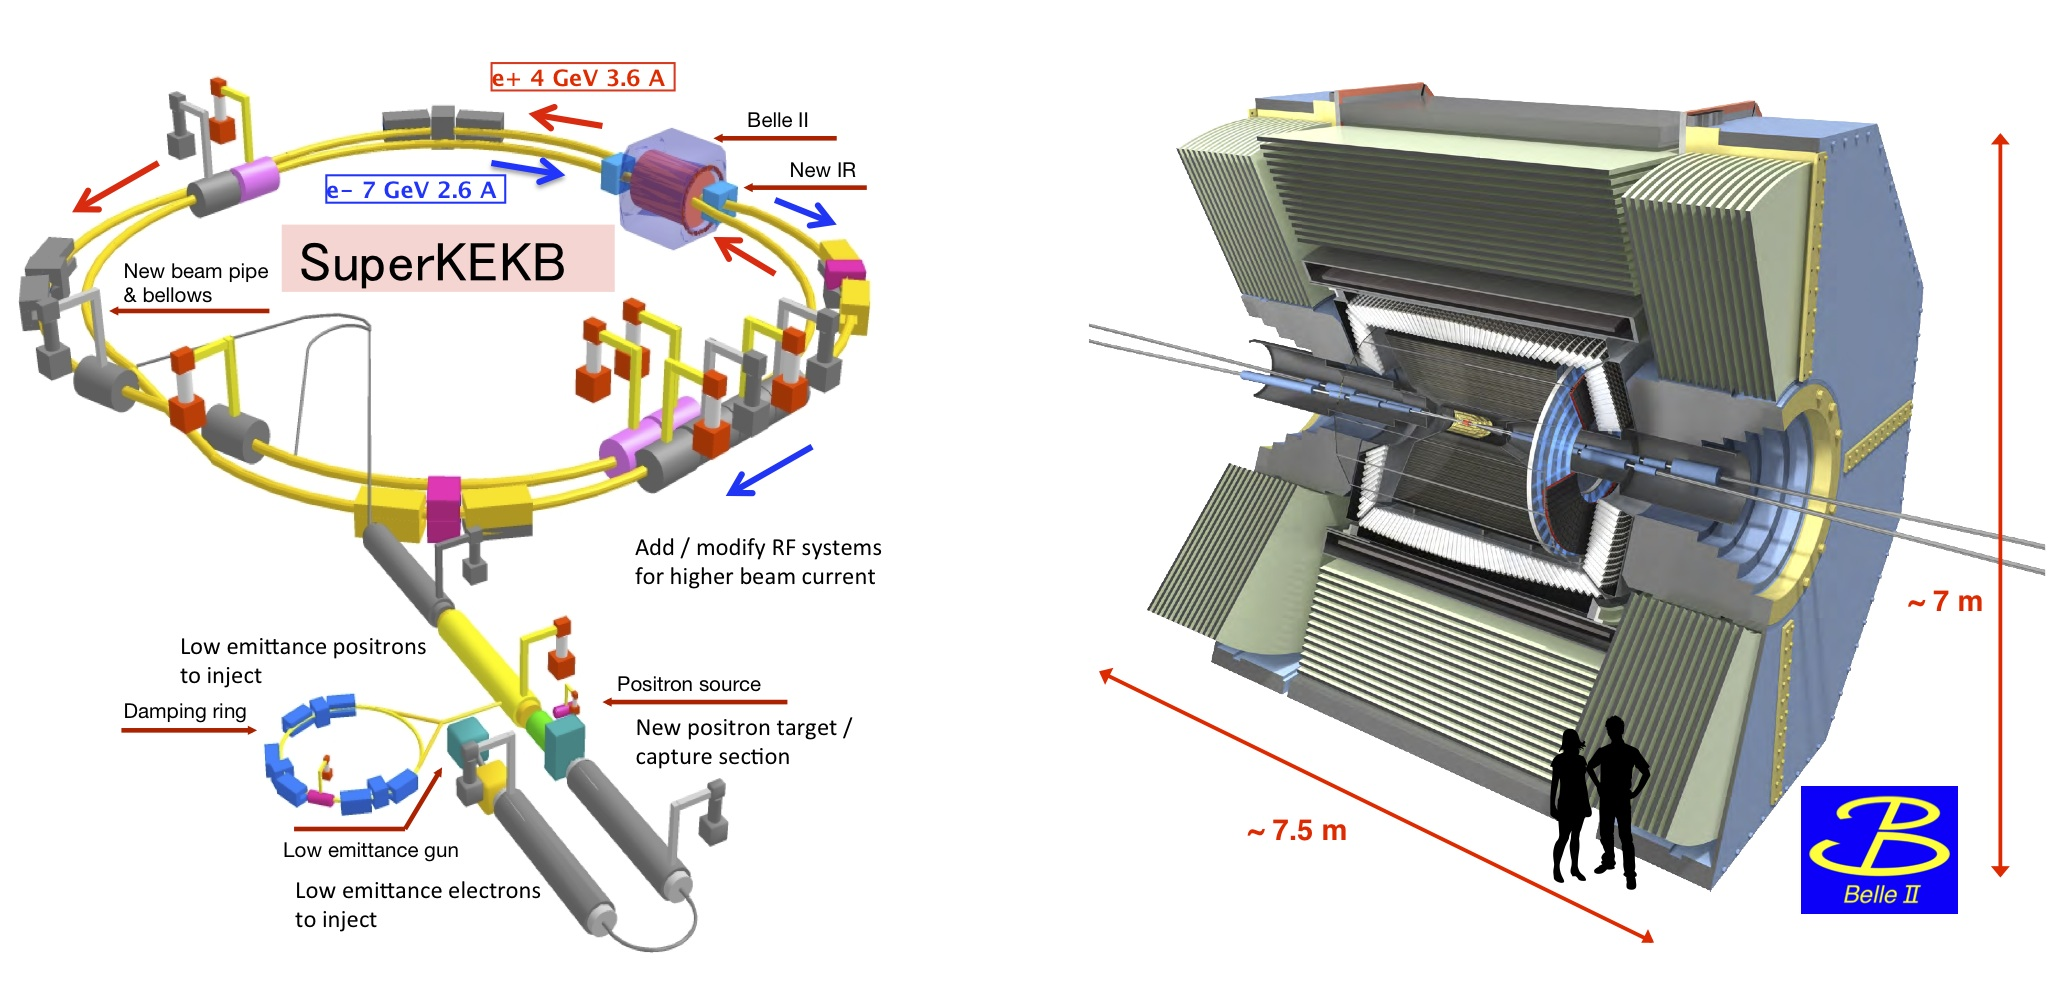
\includegraphics[width=\textwidth]{SuperKEKB_BelleII.jpg}
\end{frame}

\begin{frame}
\frametitle{Электромагнитный калориметр ECL}
  \begin{columns}
    \begin{column}{0.5\textwidth}
      \begin{itemize}
        \item 8736 \textit{CsI}(Tl) кристаллов
        \item Регистрация фотонов и электронов
        \item 20 МэВ - 8 ГэВ
        \item Монитор светимости на базе калориметра
      \end{itemize}
    \end{column}
    \begin{column}{0.5\textwidth}
      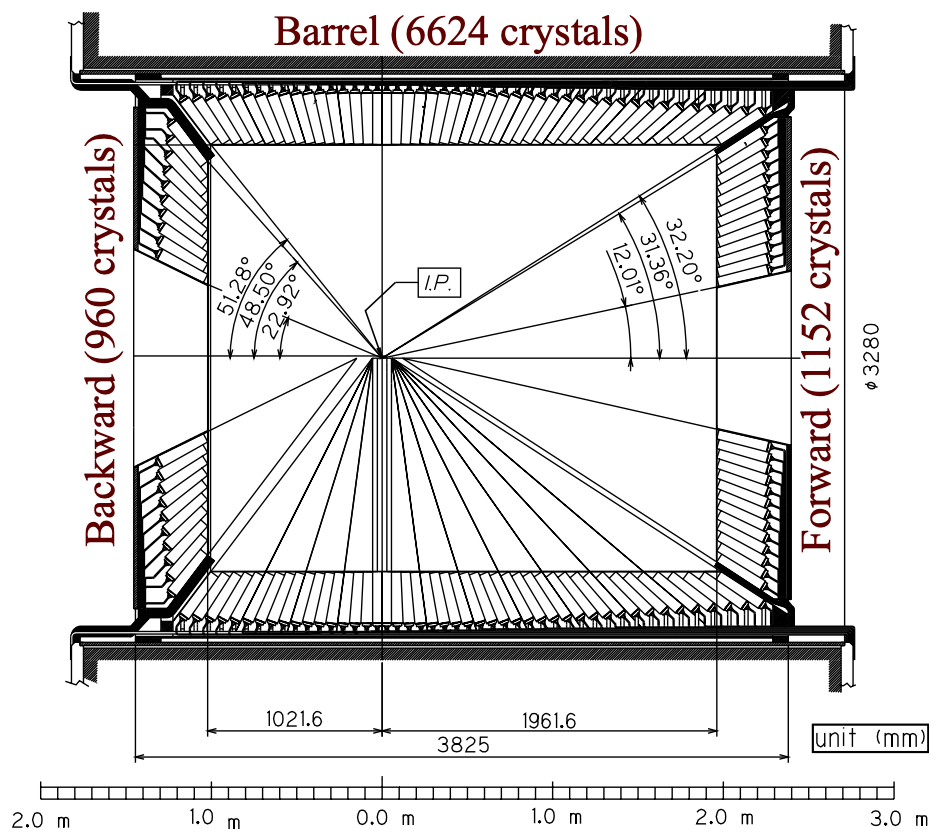
\includegraphics[width=\textwidth]{ECL}
    \end{column}
  \end{columns}
\end{frame}

\begin{frame}
\frametitle{Онлайн монитор светимости (LOM)}
\begin{columns}
  \begin{column}{0.6\textwidth}
  Разработан в институте ядерной физики
    \begin{itemize}
      \item Измеряет скорость счета $e^+e^-$ рассеяния с торцевых частей ECL
      \item Мониторирование набора данных
      \item Обратная связь с ускорителем для оптимальной настройки параметров ускорителя
      \\~\\
    \end{itemize}
    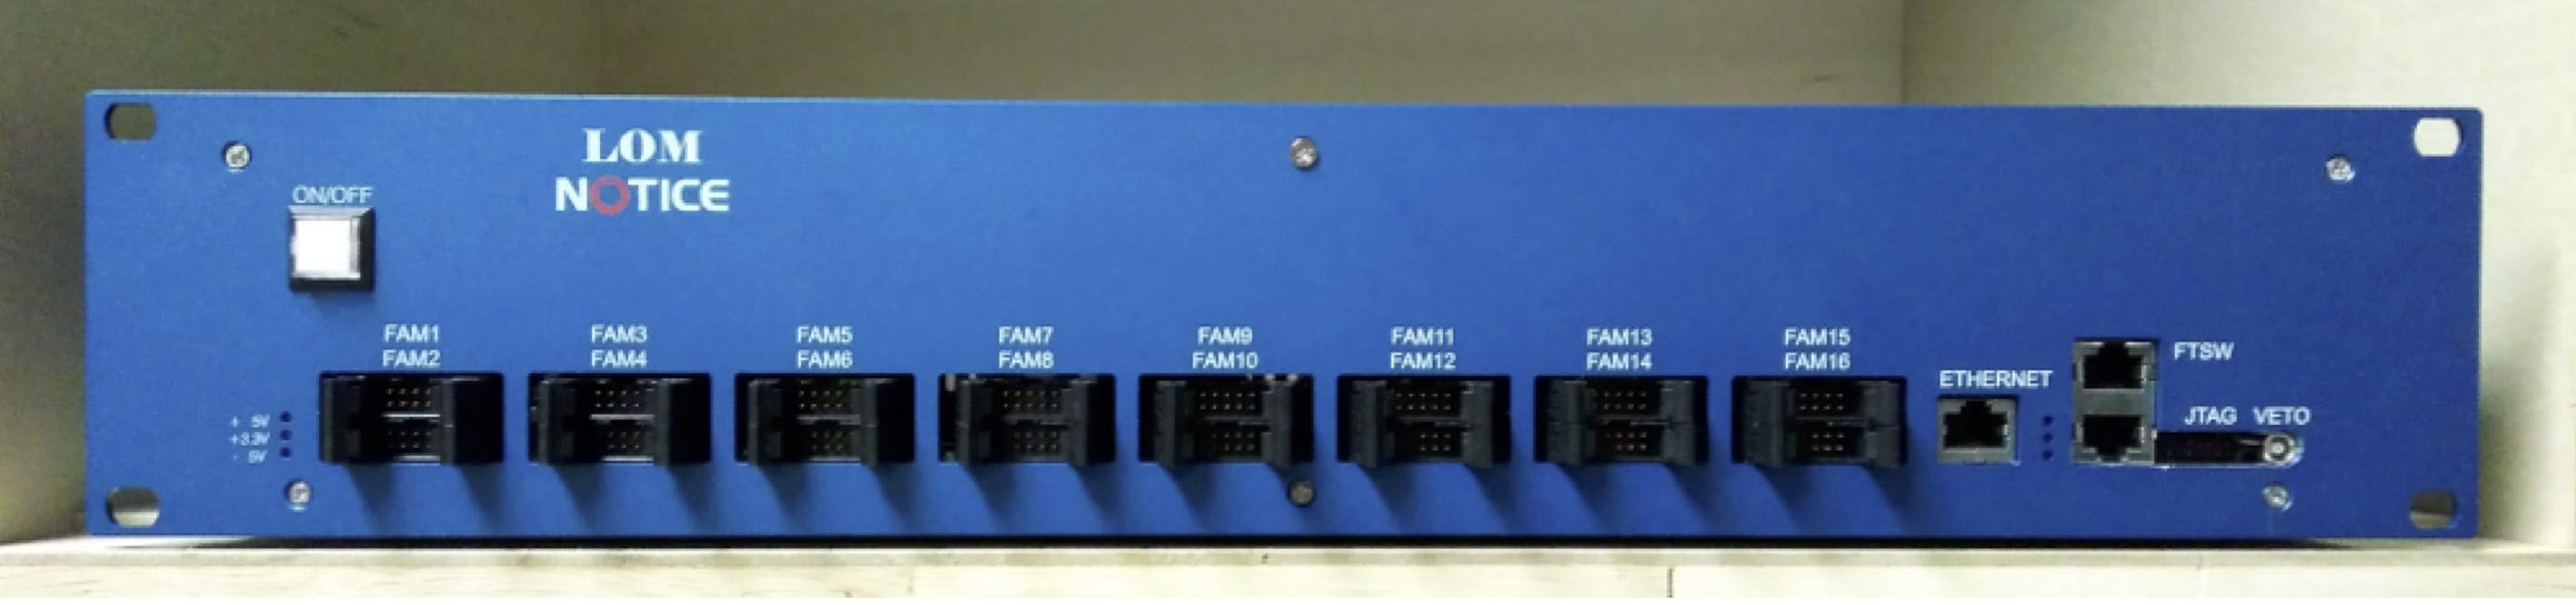
\includegraphics[width=\textwidth]{LOM_picture}
  \end{column}
  \begin{column}{0.4\textwidth}
  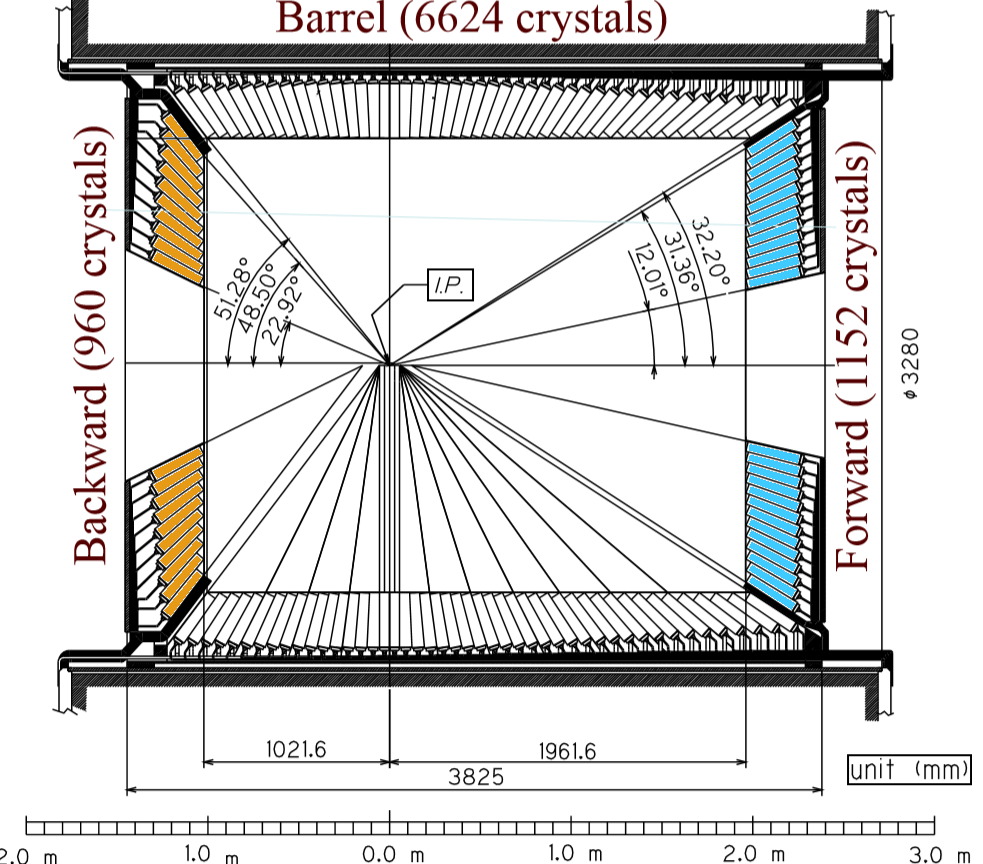
\includegraphics[width=0.85\textwidth, height=0.4\textheight]{ecl_color.png}
  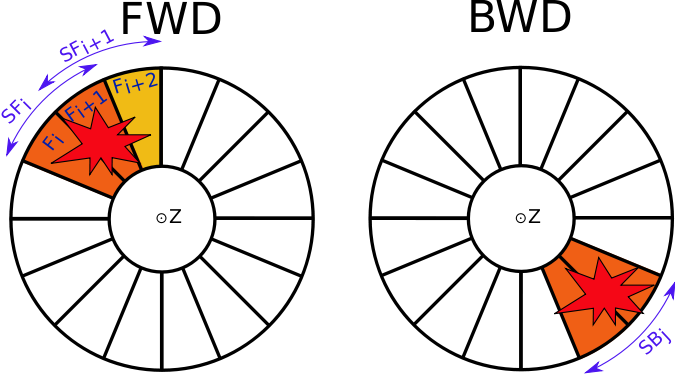
\includegraphics[width=\textwidth, height=0.3\textheight]{lom_sectors.png}
  \end{column}
\end{columns}
\end{frame}

%переписать где-то надо сказать, что именно я должен был делать
\begin{frame}
\frametitle{Задачи}
Усовершенствовать существующую версию ПО\\
  \begin{itemize}
    \item Прямая передача данных в EPICS
    \item Отображение данных (data quality monitor)
    \item Расчет интегральных и максимальных светимостей
    \item Расчет значений пьедесталов
    \item Автоматизировать процесс энергетической калибровки монитора светимости
    \item Отказоустойчивость
  \end{itemize}
\end{frame}

\begin{frame}
\frametitle{Архитектура ПО}
  \begin{itemize}
    \item Python 2.7 + библиотека pythonIOC (EPICS PV)
    \item Используются 2 системы медленного контроля NSM2 и EPICS
    \item ПО было существенно расширено и оптимизировано 
    \\~\\
  \end{itemize}
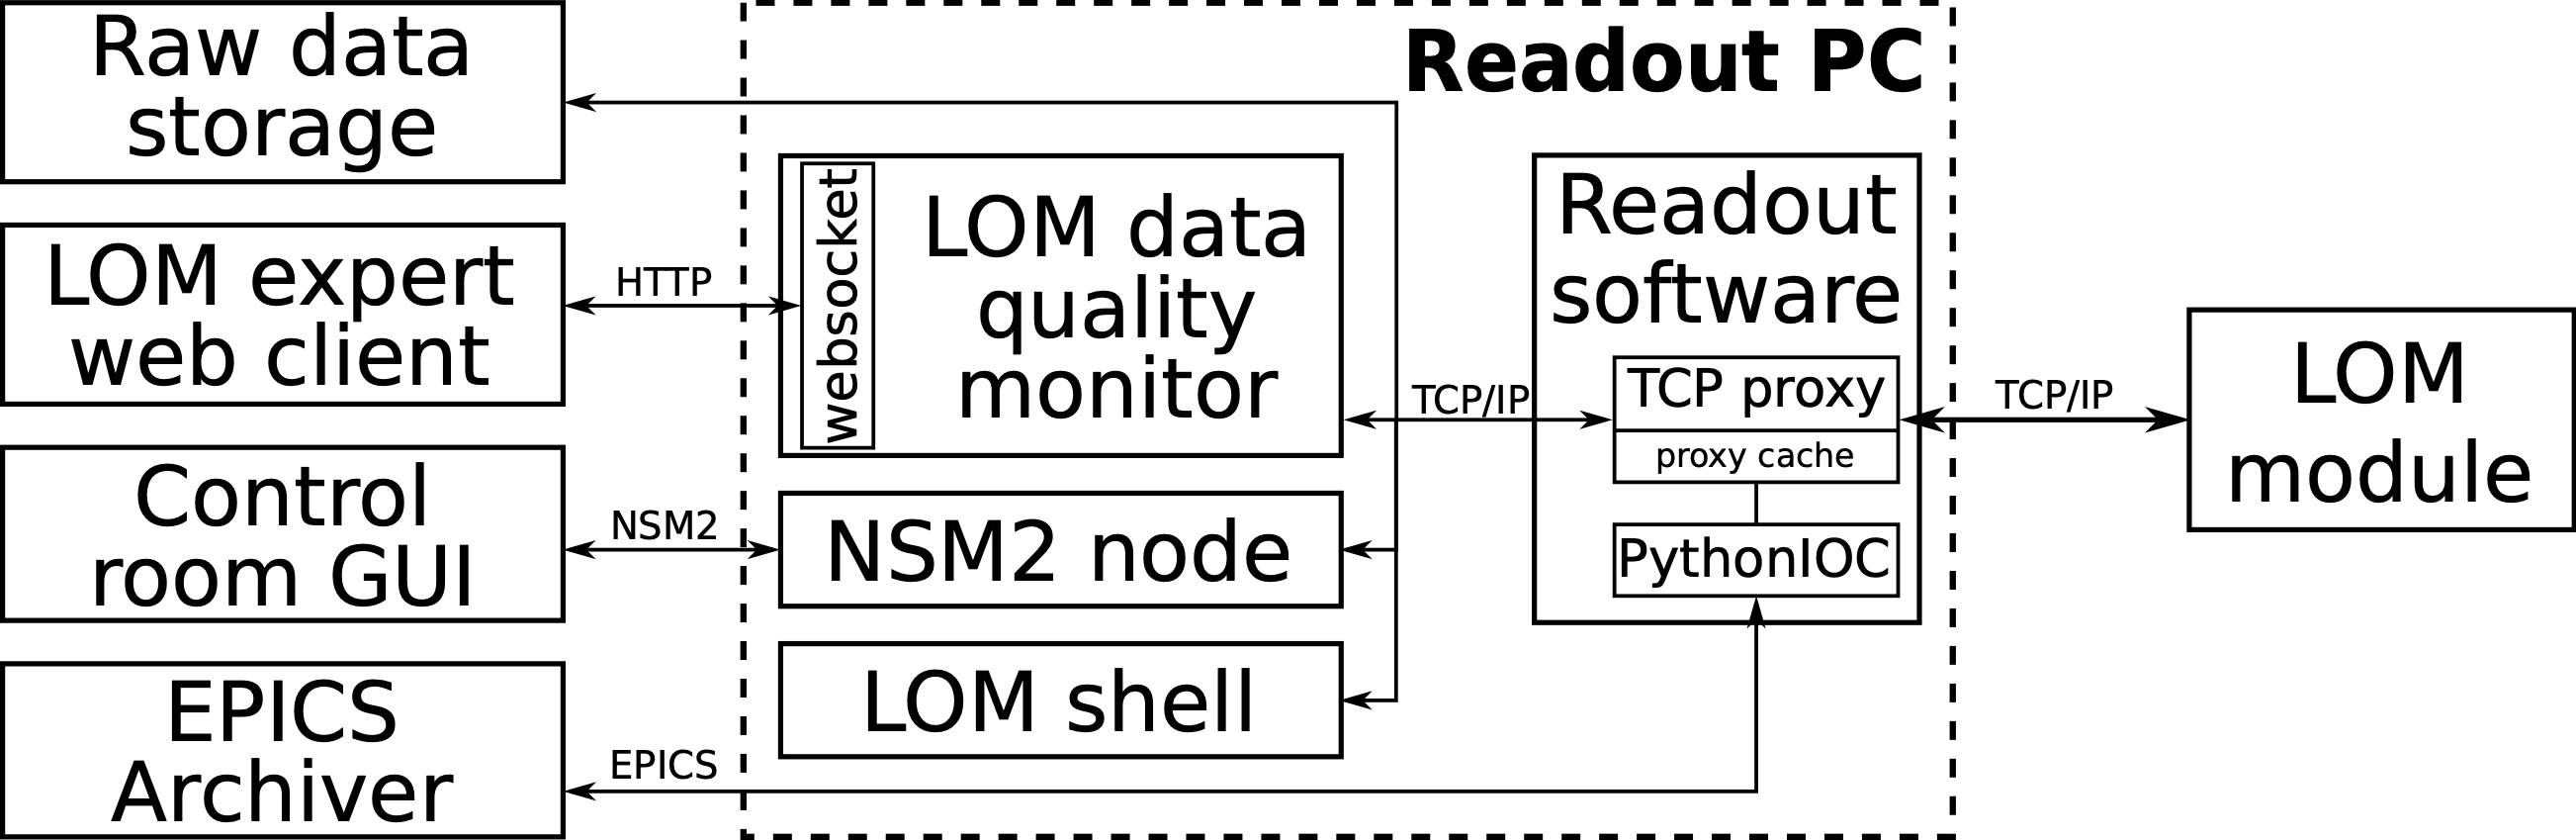
\includegraphics[width=\textwidth]{LOM_software.png}
\end{frame}

\begin{frame}
\frametitle{Система медленного контроля EPICS}
  \begin{columns}
    \begin{column}{0.5\textwidth}
      \begin{itemize}
        \item Сохранение всех значений интегральных и макисмальных значений светимости
        \item Встроенное приложение для визуализации хранящихся данных
        \item Создано 54 переменных EPICS (PV) для значений светимостей и других параметров с LOM
      \end{itemize}
    \end{column}
    \begin{column}{0.5\textwidth}
      \begin{center}
        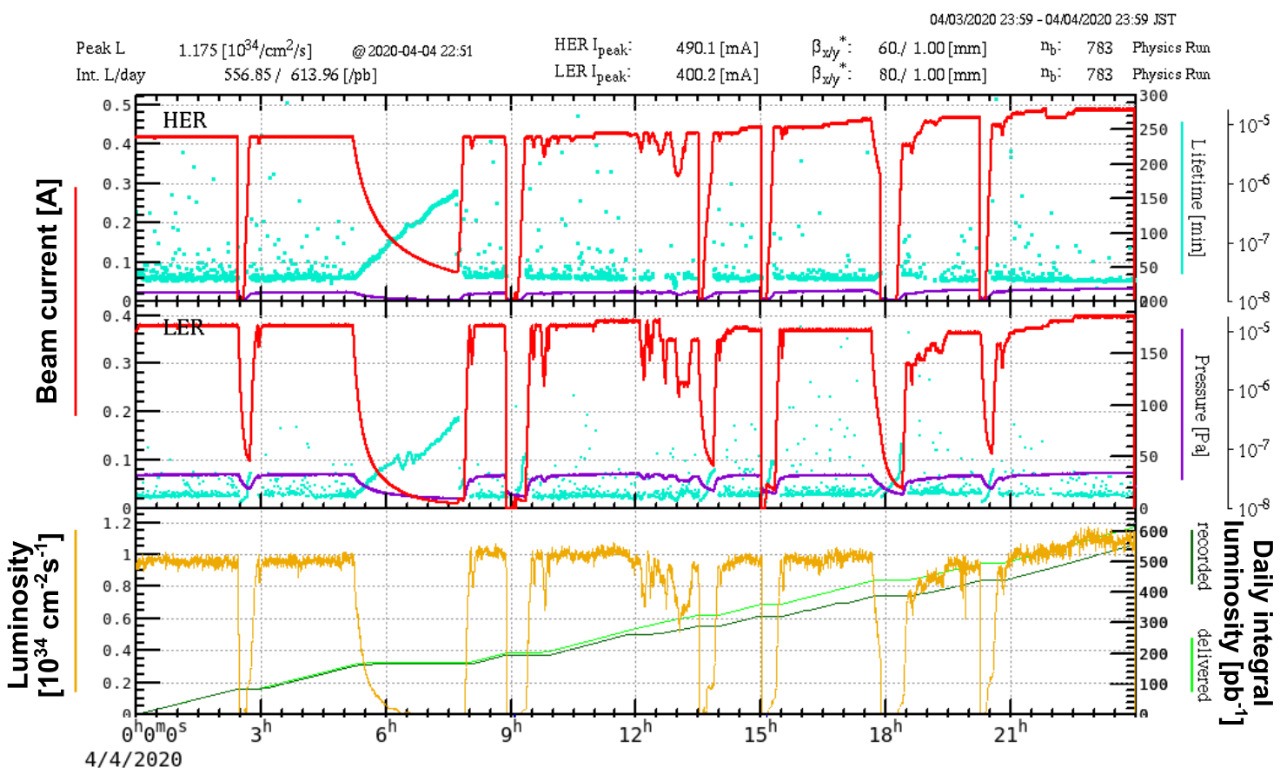
\includegraphics[width=1.0\textwidth, height=0.5\textheight]{dailysnap.jpeg}
      \end{center}
    \end{column}
  \end{columns}
  \begin{table}
    \resizebox{\textwidth}{!}{%
    \begin{tabular}{c | c | c | c }
      \thead{Мгновенная светимость} & \thead{Интегральная светимость\\по дням}  & \thead{Светимость с учётом\\ мёртвого времени детектора} & \thead{Интегральная светимость\\по заходам} \\
      \hline \hline
      \makecell{обратная связь с ускорителем} & \makecell{отображение эффективности\\работы ускорителя} & \makecell{отображение эффективности\\работы детектора} & \makecell{сравнение онлайн и\\офлайн светимости} \\ 
    \end{tabular}
    }
    %\caption{Triathlon results}
  \end{table}
\end{frame}


\begin{frame}
\frametitle{Отказоустойчивость ПО}
  Использовалась БД sqlite
  \begin{itemize}
    \item Сохранение значений светимости и даты последней модификации
    \item Сохранение значений светимости с предыдущих заходов
    \item Остановка чтения данных с монитора светимости при возникновении ошибок
  \end{itemize}
\end{frame}

\begin{frame}
\frametitle{Пьедесталы}
  \begin{itemize}
    \item Отслеживание работы калориметра
    \item Обнаружение зашумленных каналов
    \item Значения передаются в EPICS
  \end{itemize}
  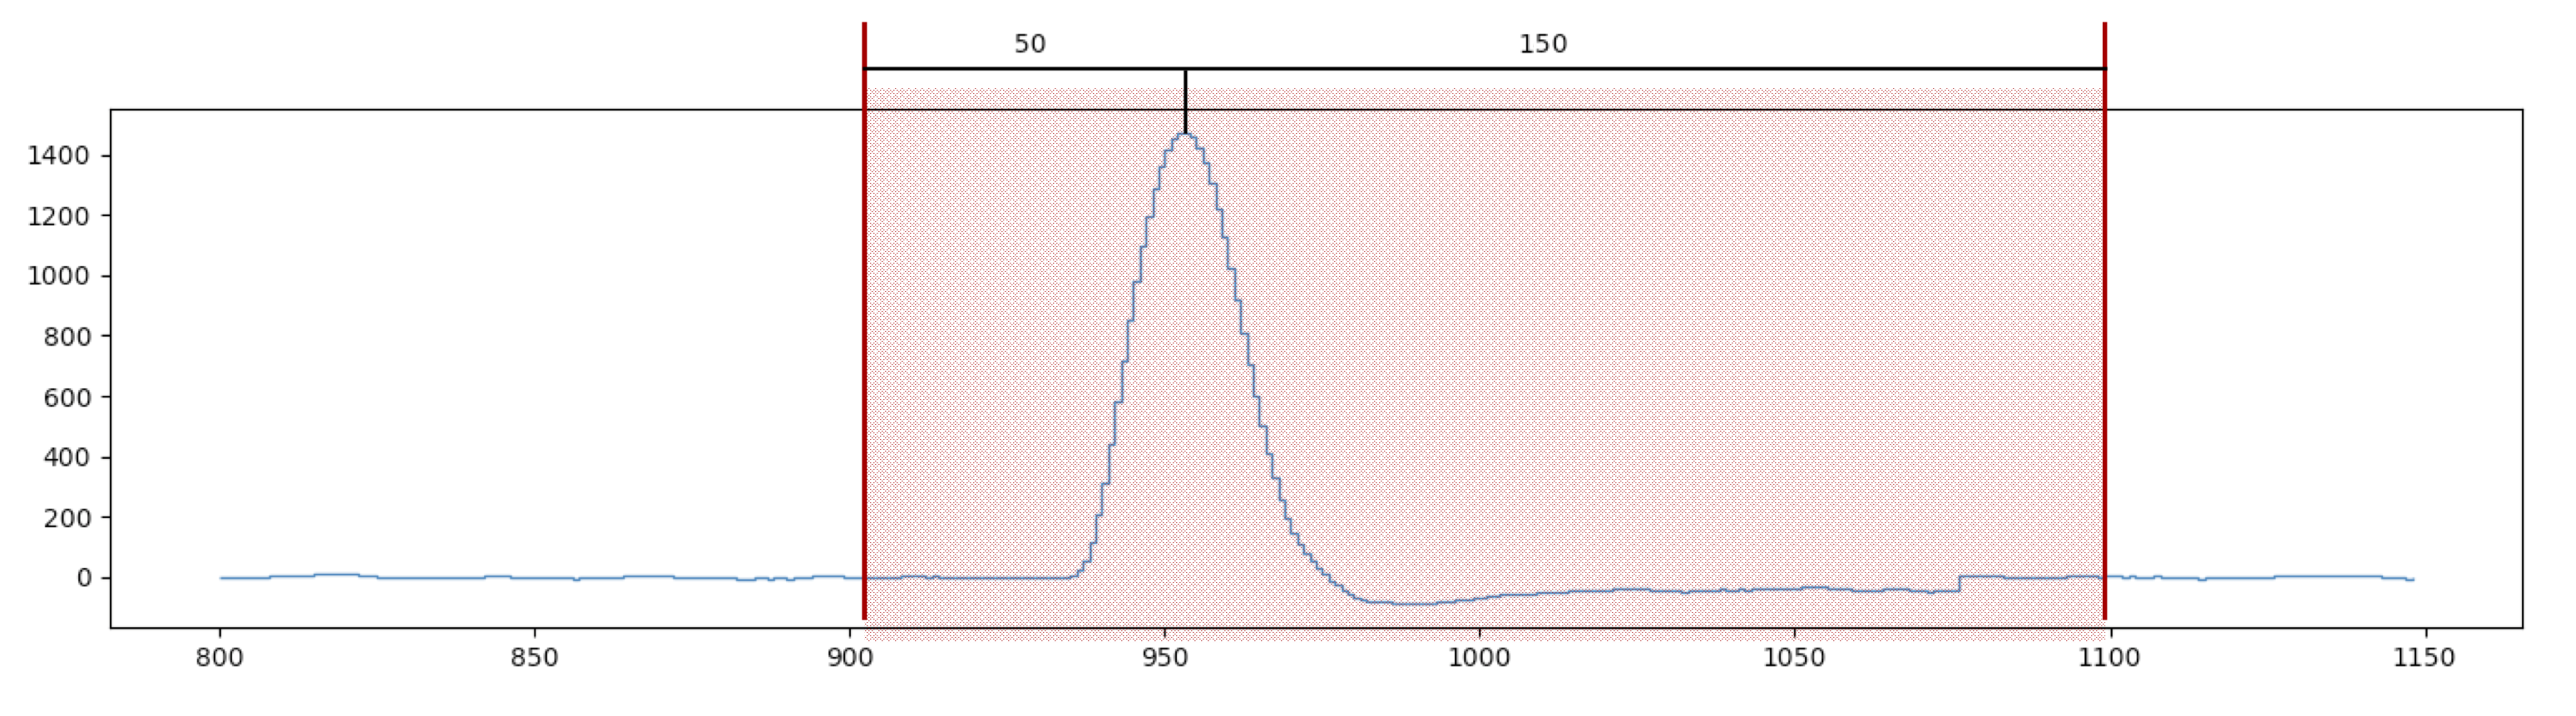
\includegraphics[width=\textwidth]{Pedestal.png}
\end{frame}

\begin{frame}
\frametitle{Data quality monitor}
  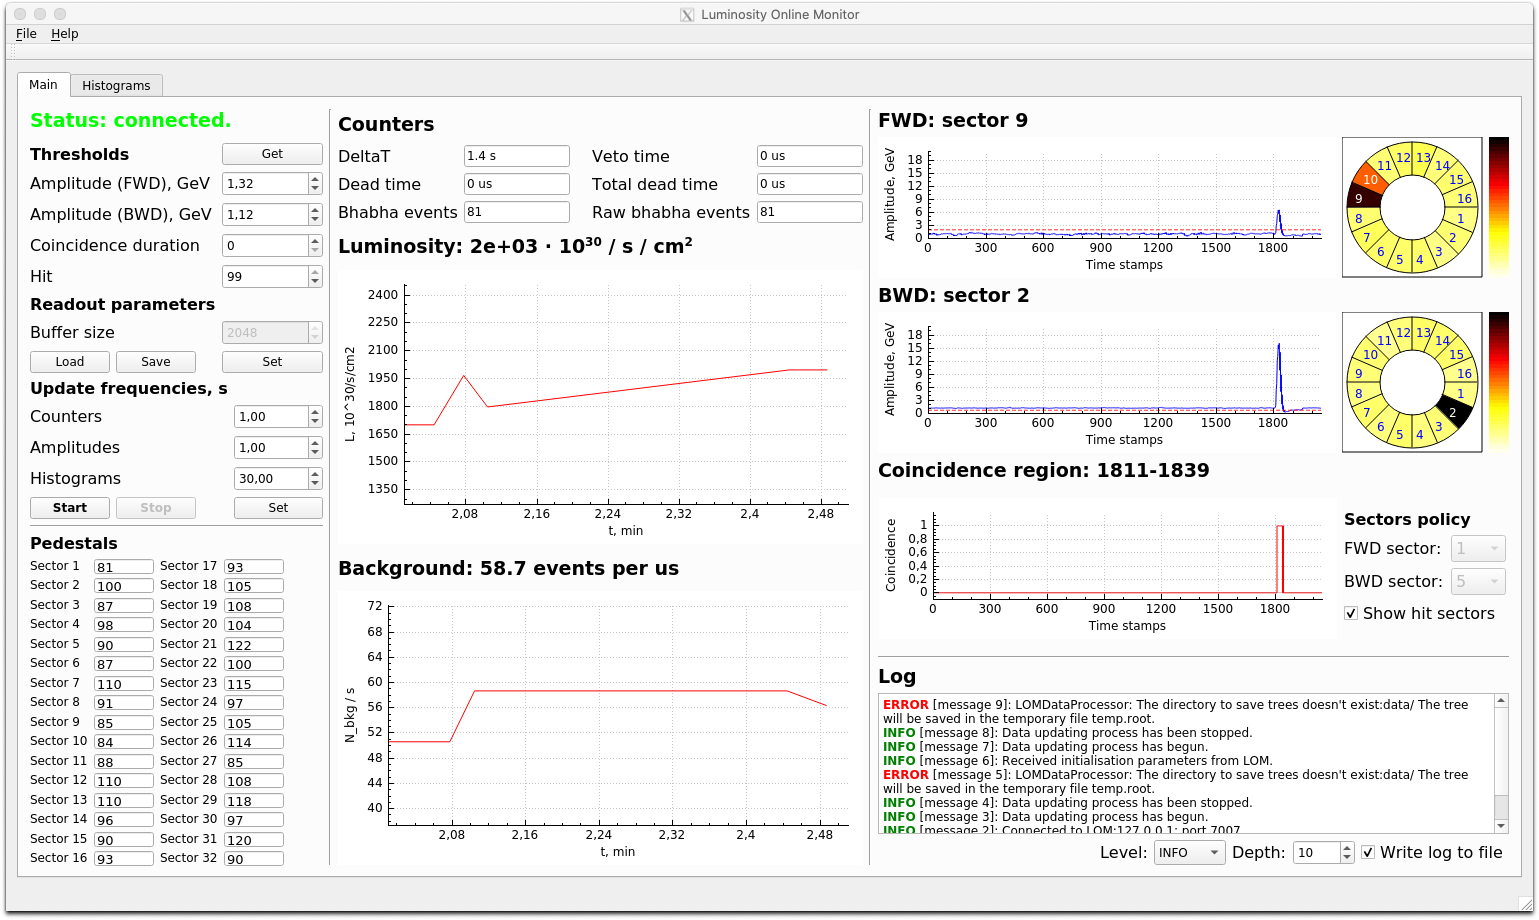
\includegraphics[width=\textwidth]{GUI3}
\end{frame}

\begin{frame}
\frametitle{Автоматизация энергетической калибровки LOM}
  \begin{center}
  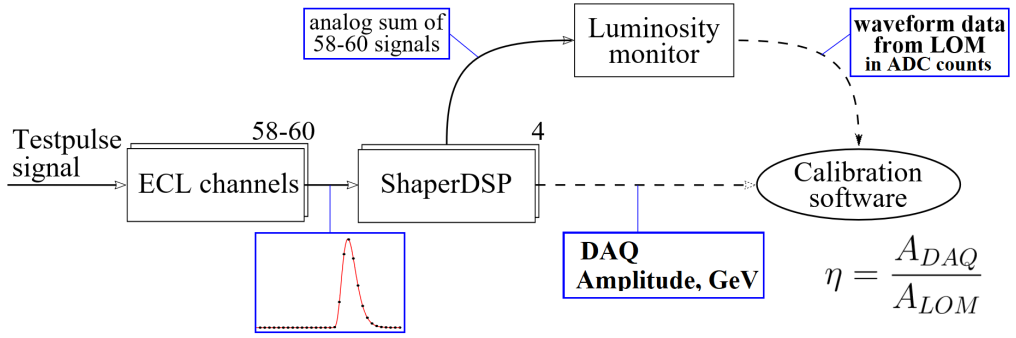
\includegraphics[width=0.75\textwidth, height=0.3\textheight]{calibration.png}
  \end{center}
  \begin{itemize}
    \item Расширен протокол управления монитором светимости
    \item Реализована возможность параллельно устанавливать конфигурацию монитора и калориметра и управлять чтением данных с соответствующих модулей
    \item Реализовано хранение калибровочных коэффициенты в БД
    \item Автоматическая подстройка калибровочных коэффицентов при изменении аттенюаторных
    \item Имеется офлайн версия калибровочных коэффициентов при отсутствии подключения к БД
  \end{itemize}
\end{frame}

\begin{frame}
\frametitle{Заключение}
  \begin{itemize}
    \item Реализовано хранение данных в системе медленного контроля EPICS
    \item Добавлен расчет интегральных и максимальных светимостей
    \item Добавлен расчет значений пьедесталов
    \item Доработан модуль data quality monitor для удаленной настройки параметров и отображения данных
    \item Усовершенствован процесс калибровки LOM
    \item Улучшено отказоустойчивость ПО
  \end{itemize}
\end{frame}

\end{document}

